\documentclass[10pt,twocolumn,letterpaper]{article}

\usepackage{cvpr}
\usepackage{times}
\usepackage{epsfig}
\usepackage{graphicx}
\usepackage{amsmath}
\usepackage{amssymb}
\usepackage{color}

% Include other packages here, before hyperref.

% If you comment hyperref and then uncomment it, you should delete
% egpaper.aux before re-running latex.  (Or just hit 'q' on the first latex
% run, let it finish, and you should be clear).
\usepackage[colorlinks=true,linkcolor=black,citecolor=black,urlcolor=black,breaklinks=true,bookmarks=false]{hyperref}

\cvprfinalcopy % *** Uncomment this line for the final submission

\def\cvprPaperID{****} % *** Enter the CVPR Paper ID here
\def\httilde{\mbox{\tt\raisebox{-.5ex}{\symbol{126}}}}

% Pages are numbered in submission mode, and unnumbered in camera-ready
%\ifcvprfinal\pagestyle{empty}\fi
\setcounter{page}{1}
\begin{document}

%%%%%%%%% TITLE
\title{ Vehicle's Lane-changing Behavior Detection and Tracking}

\author{
Mengwen He\\
CyLab-ECE\\
4720 Forbes Ave. CIC 2223G\\
{\tt\small mengwenh@andrew.cmu.edu}
% For a paper whose authors are all at the same institution,
% omit the following lines up until the closing ``}''.
% Additional authors and addresses can be added with ``\and'',
% just like the second author.
% To save space, use either the email address or home page, not both
\and
Iljoo Baek\\
CyLab-ECE\\
4720 Forbes Ave. CIC 2224G\\
{\tt\small ibaek@andrew.cmu.edu}
}

\maketitle
%\thispagestyle{empty}

%%%%%%%%% ABSTRACT
\begin{abstract}
   The lane-level localization accuracy is very important for autonomous vehicles. The Global Navigation Satellite System (GNSS), e.g. GPS, is a generic localization method for vehicles, but is vulnerable to the multi-path interference in the urban environment. Integrating the vision-based relative localization result and a digital map with the GNSS is a common and cheap way to increase the global localization accuracy and thus to realize the lane-level localization. This project is to develop a mono-camera based lane-changing behavior detection and tracking algorithm module for the correction of lateral GPS localization. We implemented a Support Vector Machine (SVM) based framework to directly classify the driving behavior, including the lane keeping, left and right lane changing, from a sampled data of the raw image captured by the mono-camera installed behind the window shield. The training data was collected from the driving around Carnegie Mellon University, and we compared the trained SVM models w/ and w/o the Principle Component Analysis (PCA) dimension reduction technique. Next, we intend to compare the SVM based classification method with the CNN method.
\end{abstract}

%%%%%%%%% BODY TEXT
\section{Introduction}

The autonomous vehicle highly relies on the accurate localization technique because it enables reliable planning and control operations for the safe autonomous driving. The Global Navigation Satellite System (GNSS), e.g. GPS, GLONASS, Beidou (Compass), and Galileo, provides commercial localization devices with affordable price but low accuracy to vehicles. It works well while driving on the highway; however, it is vulnerable to the multi-path interference caused by trees, buildings, or overhead bridges in the urban area.

The prevalent method to enhance the global localization accuracy is to use 3D Light Detection and Ranging (LiDAR) sensors, e.g. Velodyne, to conduct registration with 3D point-cloud map. This can guarantee centimeter level localization accuracy \cite{takeuchi20063} so that this method can be found on various commercial or experimental autonomous vehicles like Google, Baidu, Uber, and Toyota. However, this method is very expensive because of the 3D LiDAR and dense point-cloud map.

Therefore, the common and cheaper camera-based methods are preferred for affordable autonomous vehicles. The visual odometry method can achieve decimeter level relative localization \cite{merfels2016pose}. By implementing filter-based, e.g. Kalman filter and its variants, or graph-based, i.e. non-linear least squares, methods, we can fuse the GNSS global localization with the visual odometry relative localization to get an enhanced global result.

In this project, we want to realize a vehicle's lane-changing behavior detection and tracking algorithm based on a mono-camera. Following the integration of GNSS and camera, we want to use the road lane information from a mono-camera to enhance the global localization result; therefore, the detection and tracking of the lane-changing behavior is required to tell which lane the vehicle is on. Coupled with a digital map with road lane information, we can laterally reduce the global localization error from the GNSS as shown in Fig.\ref{fig:intro}.

\begin{figure}[t]
	\centering
	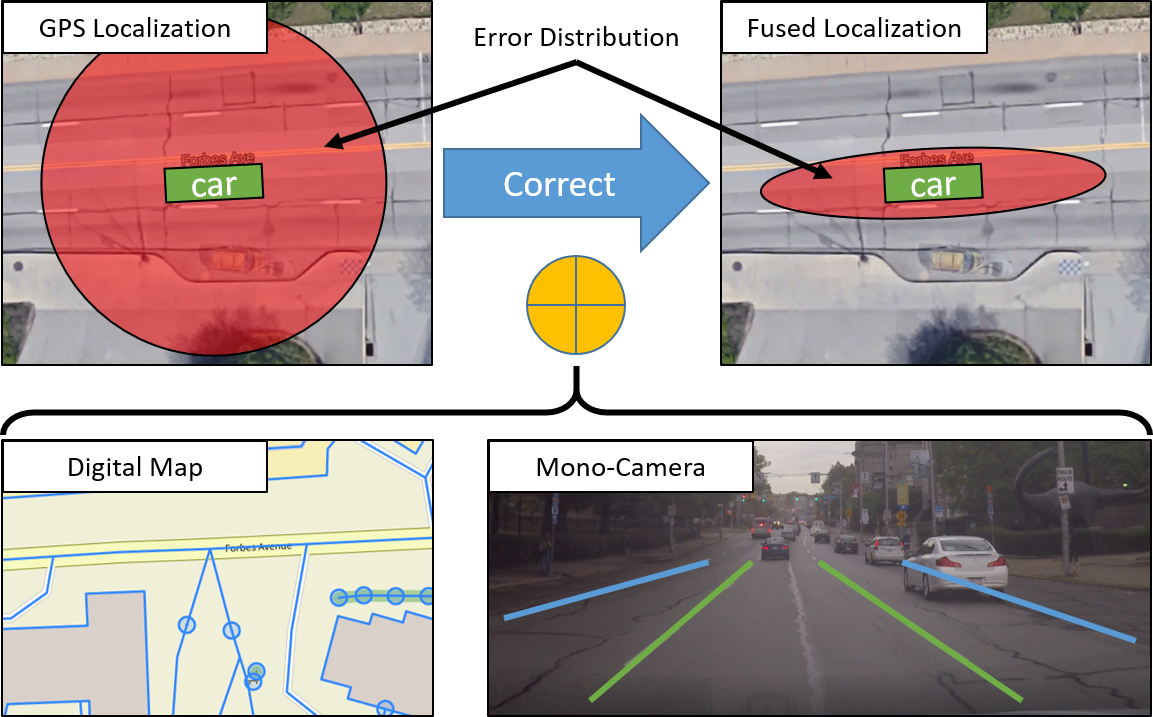
\includegraphics[width=0.4\textwidth]{./img/intro.png}
	\caption{The illustration of our project's objective. We get a global localization result from GPS with a Gaussian error model. By integrating the digital map and the lane information from our lane-changing behavior detection and tracking algorithm, we can laterally correct the global localization error.}
	\label{fig:intro}
\end{figure}

We employed a Support Vector Machine (SVM) based framework to detect the lane-changing behavior, and the training and test data/feature is directly sampled from the raw image's region-of-interest (ROI) as shown in Fig.\ref{fig:sample}. Therefore, we performed a Principle Component Analysis (PCA) dimension reduction technique to compress the feature's dimensionality as well as to keep more than $98\%$ of its original energy. 

\begin{figure}[t]
	\centering
	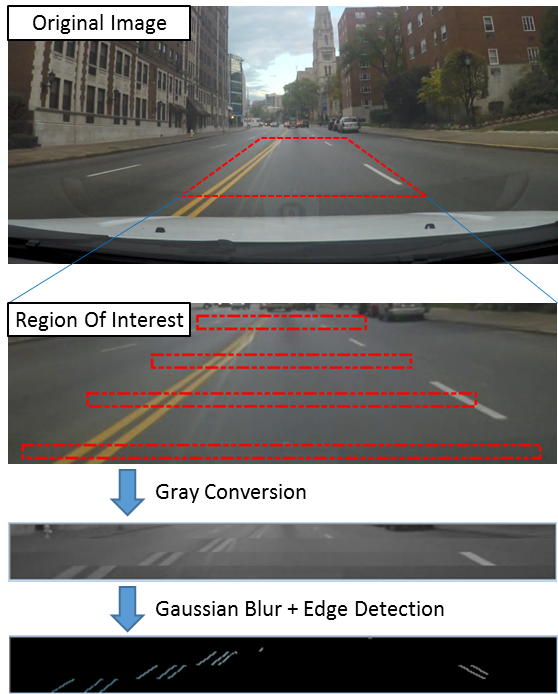
\includegraphics[width=0.45\textwidth]{./img/sample.png}
	\caption{Top: the original image with a ROI in front of the vehicle. Middle: The ROI has four sample layers (red rectangles) and each layer represents a distance (1m, 10m, 20m, 30m) from the vehicle. Bottom: Stack the sampled layers of processed pixels (edge extraction on gray image) row by row to form the feature vector.}
	\label{fig:sample}
\end{figure}

Morevoer, because of the limitation of data size, we choose to use SVM instead of the Convolution Neural Network (CNN) \footnote{18-794 Pattern Recognition Theory homework assignment 3} to classify the lane-changing behavior as lane-keeping, right lane-changing, or left lane-changing. But, we plan to compare the training results between the SVM and CNN using the same training data.

We conducted the experiment around Carnegie Mellon University with a Go-Pro HD Camera (Hero 4, $1920 \times 1080$) mounted after the window shield of Iljoo's vehicle. We used the off-the-shelf LibSVM \cite{chang2011libsvm} to train the lane-changing behavior classfier w/ or w/o PCA dimension reduction.

%------------------------------------------------------------------------
\section{Related Work}

\textcolor{red}{We have found 5 related papers \cite{mandalia2005using,pentland1999modeling,kuge2000driver,olsen2003modeling,salvucci2004inferring}, and we will finish this part after the mid-progress report.}

%-------------------------------------------------------------------------
\section{Approach and Algorithm}

\subsection{Assumptions}

For the time limitation, we make some assumptions to simplify this project; however, in the future research, we will gradually get rid of these assumptions.

\begin{itemize}
	\item This project will only work on the road with clear lane markers, and the intersection is not in its scope.
	\item The occlusion caused by other vehicles will not be considered in our training and test data.
	\item An accurate global digit map already exists and contains the lane information.
	\item The initially occupied lane is known from an upstream algorithm module.
\end{itemize}

\subsection{Training Data Collection and Labeling}

While training the SVM, it is very important to choose the most effective set of features that can represent significant differences during a lane change against lane keeping. We have tried three types of methods to collect the desired features in thie project. For the labeling, the classifier has two layers of decision as shown in Fig.\ref{fig:label}. It firstly figures out whether the vehicle changes the lane or not, and then it finds the direction of lane change.

\begin{figure}[t]
	\centering
	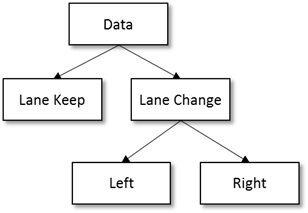
\includegraphics[width=0.3\textwidth]{./img/label.png}
	\caption{The two layer decision tree converts the three-class classification problem into a two-step binary classification problem.}
	\label{fig:label}
\end{figure}

\subsubsection{Hough Transformation Based Method}
We firstly tried to extract the lane position information by detecting lanes using open source lane detectors \cite{lanedetection,carcv}, and both of them implement the Hough transformation in the OpenCV to extract the lane edge. However, the detectors could not provide robust feature information because the ratio of true negative was too high. Additionally, the frequent false positive result (e.g. Fig.\ref{fig:lanedetection}) from the detectors has a negative impact on the SVM's performance.

\begin{figure}[t]
	\centering
	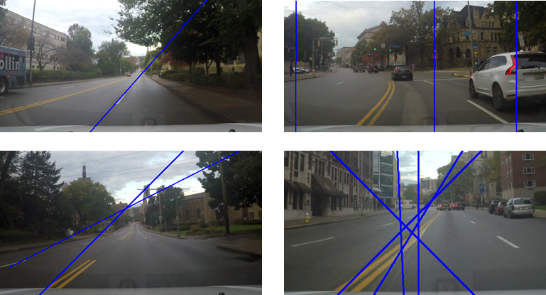
\includegraphics[width=0.45\textwidth]{./img/lanedetection.png}
	\caption{Top left/right \cite{lanedetection}:  Basic Hough transformation was conducted with canny edge detection result to find and fit lines representing the lane markers. It failed to detect the lanes in curved road scenes. Bottom left/right \cite{carcv}: Color segmentation and background subtraction were applied to extract lane marker features. Then the features were fitted into lines using the Hough transformation and contour estimation.}
	\label{fig:lanedetection}
\end{figure}

\subsubsection{Deep Neural Network Based Method}
Then we used the deep learning based SegNet tool \cite{segnet, badrinarayanan2015segnet2} to distinguish the lane markers from a road scene. However, the lane markers were often misclassified as the road in the segmentation result as shown in Fig.\ref{fig:segnet}. This is also not suitable for the SVM based classifier.

\begin{figure}[t]
	\centering
	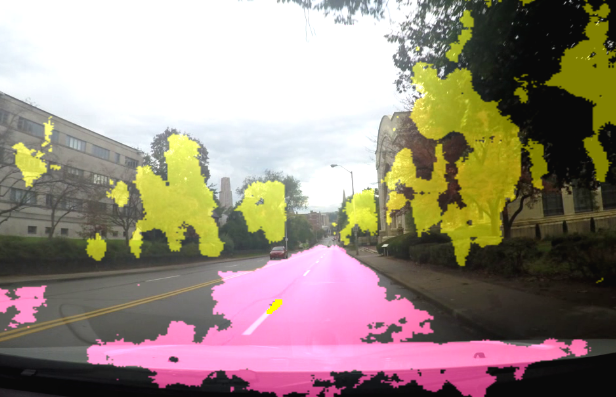
\includegraphics[width=0.4\textwidth]{./img/segnet.png}
	\caption{Each pixel in the image is classified through a sequence of non-linear processing layers (encoders) and a corresponding set of decoders followed.}
	\label{fig:segnet}
\end{figure}

\subsubsection{ROI Sampled Edge Features}
Lastly, we tried to extract the binary edge information from a pre-defined ROI as shown in Fig.\ref{fig:sample}. The ROI has four layers and each layer represents a distance (1m, 10m, 20m, 30m) from the vehicle. The ROI pixels are converted to gray, blurred by Gaussian, and filtered by Canny Edge detector. According to our test, these binary edge features are robust and stable enough to provide continuous information for the SVM classifier.

\subsection{PCA Dimension Reduction}

The training data/feature's dimensionality is 16,000; therefore, we want to use the PCA to shrink its dimensionality and focus on the main components. Moreover, because the dimensionality is greatly larger than the data size, we will use the Gram Matrix Trick to accelerate the eigen decomposition operation.

\subsubsection{Gram Matrix Trick}

Given a centralized training data matrix $X$ with dimension $d \times N$, we derive its covariance matrix as $\Sigma=E(XX^{T})$. The PCA needs to solve the problem as below:
\begin{equation}
\begin{array}{rcl}
\Sigma \vec{v} & = & \lambda \vec{v} \\
XX^T\vec{v} & = & \lambda' \vec{v} \\
X^TXX^T\vec{v} & = & \lambda' X^T \vec{v} \\
X^TX\vec{v}' & = & \lambda'' \vec{v}'~~~~(\vec{v}'=\eta X^T\vec{v}) \\
\end{array}
\end{equation}
Therefore, we only need to solve the eigen decomposition of the Gram matrix $X^TX$ with dimension $N \times N$. To get the final eigenvectors $\{\vec{v}_i\}$, we need to solve:
\begin{equation}
\left\{\begin{array}{rcl}
XX^T\vec{v} & = & \lambda' \vec{v} \\
\vec{v}' & = & \eta X^T \vec{v} \\
\end{array}\right. \Rightarrow \vec{v}=\eta' X\vec{v}'
\end{equation}
Then we can use $\Sigma\vec{v}=\lambda\vec{v}$ to derive all the corresponding eigenvalues $\{\lambda_i\}$.

\subsubsection{Dimension Reduction}

Firstly, We sort the derived eigenvalues (associated with the corresponding eigenvectors) in a descending order, and we calculate the total energy as below:
\begin{equation}
\Lambda=\sum_{i=1}^{d}{\lambda_i}
\end{equation}
Then, we choose the first $M$ biggest eigenvalues whose summation is just larger than a threshold ratio $r$ of the total energy $\Lambda$.
\begin{equation}
\begin{array}{rcl}
\sum_{i=1}^{M}{\lambda_i} & \geq & r\Lambda \\
\sum_{i=1}^{M-1}{\lambda_i} & < & r\Lambda \\
\end{array}
\end{equation}
Finally, we use the first $M$ biggest eigenvalues' corresponding eigenvectors to form a PCA dimension reduction matrix $P$ as below:
\begin{equation}
P=[\vec{v}_1,\dots,\vec{v}_M]
\end{equation}
Therefore, the dimension reduced new centralized trainidng data matrix is $X'=P^TX$. If we use the PCA dimension reduction on the training data as well as the SVM, we also need to apply the dimension reduction on the test data $Y$ following these two steps:
\begin{enumerate}
	\item Centralize the test data with the mean ($\mu_X$) of the training data.
	\item Reduce its dimension to get $Y'=P^T(Y-\mu_X)$
\end{enumerate}

\subsection{LibSVM Training and Test}

The LibSVM already provides some off-the-shelf applications to conduct and evaluate the binary classification, and what we need to provide is the training and test data following the format required by the LibSVM. The data is stored in ASCII format, and each row in it presents a labeled feature. Because the LibSVM supports sparse matrix operations, the labeled feature is stored as a label followed with a sequence of indexed non-zero values as below:

\begin{verbatim}
-1 1:1 11:1 18:1 20:1 37:1 42:1 59:1 
+1 5:1 18:1 19:1 39:1 40:1 63:1 
\end{verbatim}

\subsection{Lane Changing Behavior Tracking}

\textcolor{red}{Not done yet, will be finished after the mid-progress report.}

%-------------------------------------------------------------------------
\section{Experiments and Progress}

The implementation pipeline of this project is shown as Fig.\ref{fig:pipeline}.

\begin{figure}[t]
	\centering
	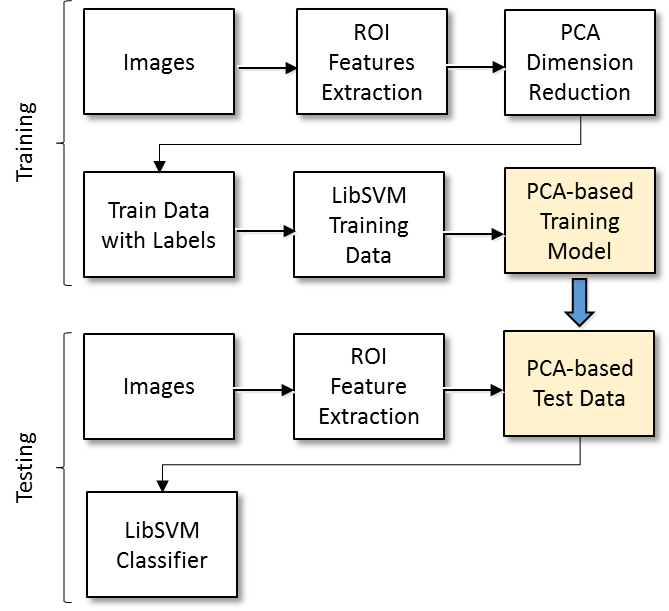
\includegraphics[width=0.4\textwidth]{./img/pipeline.png}
	\caption{The pipeline of this SVM based lane-changing behavior detection project.}
	\label{fig:pipeline}
\end{figure}

\subsection{Data Collection and Labeling}

A tool shown in Fig.\ref{fig:tool} was developed to create the training and ground truth data. We defined three classes which are `Lane Keep', `Lane Change - Left', and `Lane Change- Right'. The class type is manually determined, and the feature data is automatically labeled using the user interface provided by this tool. The binary edge feature presents the distinguishing pattern between two class types as shown in Fig.\ref{fig:feature}.

\begin{figure}[t]
	\centering
	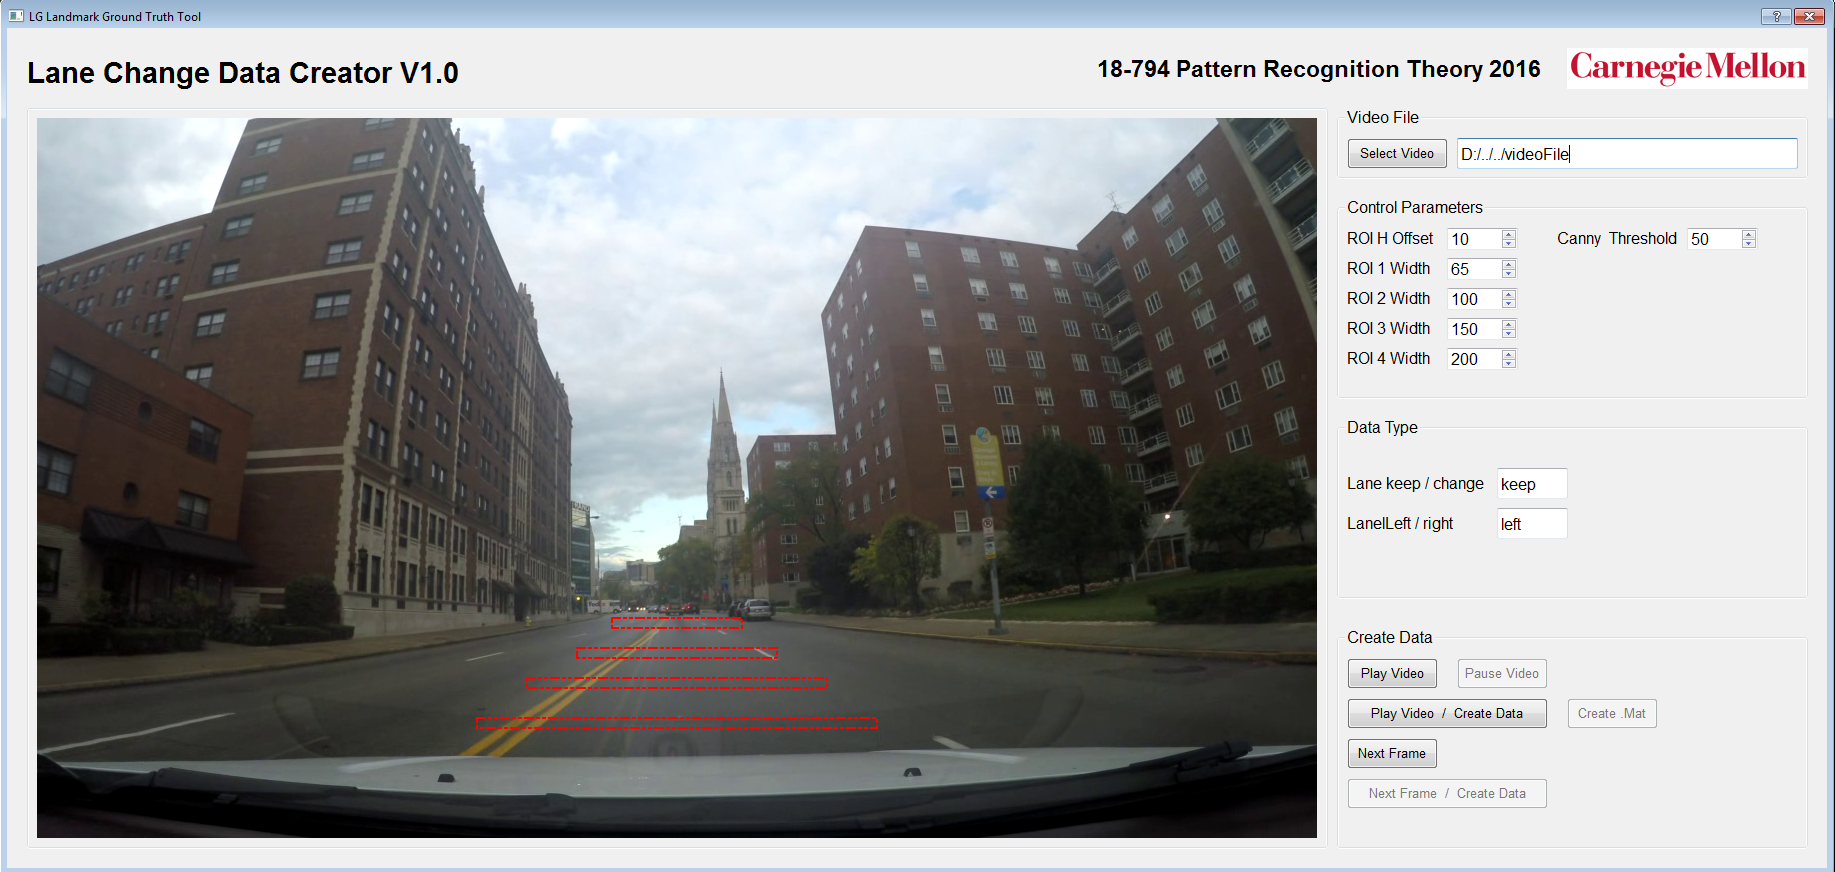
\includegraphics[width=0.5\textwidth]{./img/tool.png}
	\caption{The tool to collect data and extract feature.}
	\label{fig:tool}
\end{figure}

\begin{figure}[t]
	\centering
	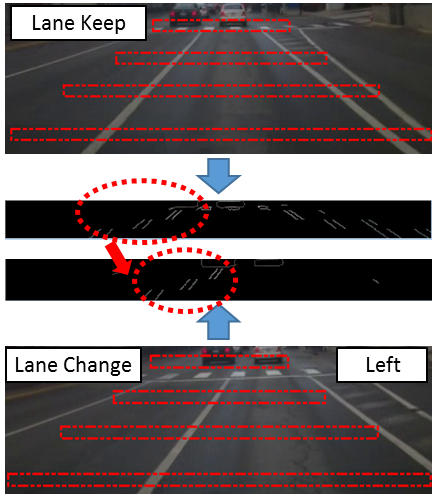
\includegraphics[width=0.45\textwidth]{./img/feature.png}
	\caption{Compare the features extracted from the `Lane Keep' behavior and the `Lane Change - Left' behavior.}
	\label{fig:feature}
\end{figure}

\subsection{SVM Training Result}

The training and test data are collected from the roads around Carnegie Mellon University as shown in Fig.\ref{fig:datamap}.  From these two roads, we extracted and labeled $321$ training data and $285$ test data. Then we present the training results as two groups: w/o PCA dimension reduction v.s. w/ PCA dimension reduction, and for each group, we also present the training results as two subgroups: w/o RBF kernel v.s. w/ RBF kernel.

\begin{figure}[t]
	\centering
	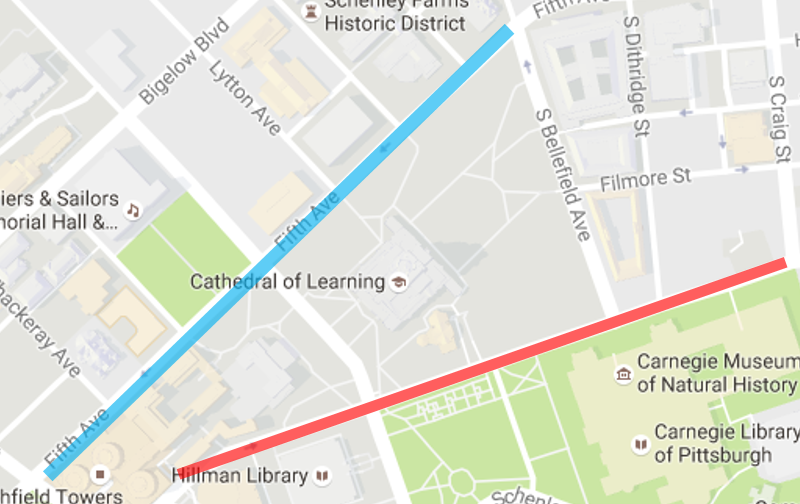
\includegraphics[width=0.4\textwidth]{./img/datamap.png}
	\caption{The locations where we collect the training data (blue) and test data (red).}
	\label{fig:datamap}
\end{figure}

\subsubsection{Without PCA Dimension Reduction}

\paragraph{Without RBF kernel}

\begin{itemize}
	\item Train data: $16,000 \times 321$ (dimension $\times$ data size)
	\item Test data: $16,000 \times 285$
	\item Accuracy: $88.0702\%~(251/285)$
	\item Confusion matrix: Tab.\ref{tb:cm1}
\end{itemize}

\begin{table}
	\caption{Confusion Matrix w/o PCA, w/o RBF}
	\label{tb:cm1}
	\begin{tabular}{|c|c|c|}
		\hline
		& Lane Keeping & Lane Changing \\
		\hline
		Lane Keeping & 159 & 19 \\
		\hline
		Lane Changing & 15 & 92 \\
		\hline
\end{tabular}
\end{table}

Because the feature is already in high-dimensional space, the linear SVM's accurate rate, $88\%$, is acceptable with a small size of training data.

\paragraph{With RBF kernel}

\textcolor{red}{Currently, we did not use the kernel in our experiment, and we will implement it after the mid-progress report.}

\subsubsection{With PCA Dimension Reduction}

\paragraph{Without RBF kernel}

\begin{itemize}
	\item PCA energy: $>98\%$
	\item PCA Train data: $154 \times 321$
	\item PCA Test data: $154 \times 285$
	\item Accuracy: $62.4561\%~(178/285)$
	\item Confusion matrix: Tab.\ref{tb:cm2}
	

\end{itemize}

\begin{table}
	\caption{Confusion Matrix w/ PCA, w/o RBF}
	\label{tb:cm2}
	\begin{tabular}{|c|c|c|}
	\hline
	& Lane Keeping & Lane Changing \\
	\hline
	Lane Keeping & 178 & 0 \\
	\hline
	Lane Changing & 107 & 0 \\
	\hline
\end{tabular}
\end{table}

After PCA dimension reduction, the feature is in a low-dimensional space; therefore, the linear SVM's accurate rate, $62\%$, significantly reduced compared to the result without PCA and RBF kernel. Actually, from the confusion matrix, we find this SVM classifier does not work, because the output is always `Lane Keeping'. Therefore, we assert that the dimension reduced feature is not linear-separable, and the kernel is required to increase its performance.

\paragraph{With RBF kernel}

\textcolor{red}{Currently, we did not use the kernel in our experiment, and we will implement it after the mid-progress report.}

\subsection{CNN Training Result}

\textcolor{red}{Not done yet, will be finished after the mid-progress report.}

%-------------------------------------------------------------------------
\section{Conclusion}

\textcolor{red}{Not done yet, will be finished after the mid-progress report.}

%-------------------------------------------------------------------------

{\small
\bibliographystyle{ieee}
\bibliography{egbib}
}

\end{document}
